%==========================================================================
% Exemplo de artigo cientifico UNESC
%
% v0.0 versão em 20/09/2023 por Marlon Oliveira
% v1.0 versão em 25/06/2025 por Marlon Oliveira


%==========================================================================

%==========================================================================
% Pacotes utilizados pela UNESC - não delete as linhas abaixo
%==========================================================================
\documentclass{UNESC}
\usepackage[T1]{fontenc}
\usepackage[utf8]{inputenc}%\usepackage[latin1]{inputenc}
\renewcommand{\rmdefault}{phv} % Arial
\renewcommand{\sfdefault}{phv} % Arial
\usepackage[brazilian]{babel}
\usepackage{graphicx}
%\usepackage{subfigure}
\usepackage{hyperref}
\usepackage{quoting}
\usepackage[labelsep=none]{caption}
\DeclareCaptionLabelFormat{figuracomtraco}{#1~#2 -}
\captionsetup[figure]{labelformat=figuracomtraco, labelsep=space}
\captionsetup[table]{labelformat=simple, labelsep=space, textformat=simple}
\DeclareCaptionLabelFormat{tabelacomtraco}{#1~#2 -}
\captionsetup[table]{labelformat=tabelacomtraco}
\captionsetup{labelsep=none}
%\renewcommand{\thefigure}{\arabic{figure} - }
\usepackage{enumitem}
\usepackage{float}
\usepackage{comment}
\usepackage[hang,flushmargin]{footmisc}
\usepackage{array}
\usepackage{adjustbox}

\hypersetup{
  setpagesize  = false,
  colorlinks   = true,    % Colours links instead of ugly boxes
  urlcolor     = blue,    % Colour for external hyperlinks
  linkcolor    = black,   % Colour of internal links
  citecolor    = black    % Colour of citations
}

\urlstyle{same}
\usepackage{setspace}

\usepackage[alf,recuo=0.0cm,abnt-emphasize=bf]{abntex2cite} 

%\captionsetup[figure]{justification=raggedright}


%==========================================================================
% Dados do artigo: título, autores e filiação
%==========================================================================
\title{REGISTRO DIGITAL ANIMAL: DIGITALIZANDO A IDENTIFICAÇÃO E CONTROLE DE VACINAÇÃO DE ANIMAIS DE ESTIMAÇÃO}
\author
{
   Gabriel Goulart de Souza\footnote{Curso de Ciência da Computação, Universidade do Extremo Sul Catarinense (Unesc), Criciúma - Santa Catarina - Brasil. gabriel.gsouzza6@unesc.net},
   Diorgines Mattos Machado\footnote{Coorientador(a), Curso de Ciência da Computação, Universidade do Extremo Sul Catarinense (Unesc), Criciúma - Santa Catarina - Brasil. diorginesmattos@unesc.net},
   Allan Farias Favaro\footnote{Orientador(a), Curso de Ciência da Computação, Universidade do Extremo Sul Catarinense (Unesc), Criciúma - Santa Catarina - Brasil. allanfavaro@gmail.com}
}

%==========================================================================
% Início do texto do artigo
%==========================================================================
\begin{document}

\onehalfspacing

\maketitle

\noindent
\textbf{Resumo:} Deve ter uma sequência de frases concisas e objetivas em parágrafo único, sem enumeração de tópicos, de 100 a 250 palavras, seguido, logo abaixo, das palavras representativas do conteúdo do trabalho, isto é, palavras-chave e/ou descritores, conforme a \citeonline{ABNT2021}.

\vspace{0.5em}
\noindent
\textbf{Palavras-chave:} Elemento obrigatório. Devem ser separadas entre si por ponto e vírgula e finalizadas por ponto, com as iniciais em letra minúscula, com exceção dos substantivos próprios e nomes científicos. 

\vspace{1.0em}
\noindent
\textbf{ABSTRACT:} Tradução do resumo em língua vernácula para outro idioma de propagação internacional (em inglês ABSTRACT, em francês RESUMÉ, em espanhol RESUMEN).

\vspace{0.5em}
\noindent
\textbf{Keywords:} keyword 1; keyword 2; keyword 3.


\section{INTRODUÇÃO}

% A introdução apresenta o assunto, delimita o tema e analisa a problemática a ser investigada, com as questões norteadoras e as hipóteses formuladas. Nela devem constar também os objetivos da pesquisa, a justificativa da escolha do tema e a metodologia utilizada.

% Consiste no que se deseja atingir com o desenvolvimento da pesquisa, deve evidenciar de forma genérica o propósito mais amplo da realização do trabalho. O objetivo da pesquisa tanto o geral quanto os específicos devem ser bem definidos, já que se refere ao que será alcançado com a finalização do trabalho. Objetivos geral inicia por verbo no infinitivo.


% Os objetivos específicos são o detalhamento do objetivo geral, devendo refletir o que se espera do trabalho em relação aos aspectos computacionais e ao domínio de aplicação. Estes objetivos devem ser passíveis de realização, considerando-se o tempo disponível para realização da pesquisa. Objetivos específicos iniciam por verbo no infinitivo.
% Deve-se escrever sobre os motivos que determinaram a escolha do tema da pesquisa, destacando-se a relevância computacional, bem como do domínio de aplicação. 
% Para facilitar o processo de redação da justificativa, deve-se perguntar: \\
% -	O tema é relevante? Por quê? 

% -	Quais os pontos positivos da abordagem a ser pesquisada? 

% -	Que vantagens/benefícios esta pesquisa pode proporcionar? 

% Exemplo de citação de referência: \cite{gandini2002} ou \citeonline{gandini2002}
% Citação de site: \cite{unep}
% A seguir, um exemplo com citação direta longa. \\


% \begin{quoting}[rightmargin=0cm,leftmargin=4cm]
% \begin{singlespace}
% {\footnotesize \noindent
% A performance se estrutura, portanto, numa linguagem “cênico-teatral” e é apresentada na forma de um mixed-media onde a tonicidade maior pode dar-se um uma linguagem ou outra, dependendo da origem do artista (mais plástica no Fluxus, mais teatral em Disappearances).} 
% \end{singlespace}
% \end{quoting}

% Caso tenha fórmulas ou equações, para facilitar a leitura, devem ser destacadas no texto e, se necessário, numeradas com algarismos arábicos entre parênteses, alinhados à direita. Na sequência normal do texto, é permitido o uso de uma entrelinha maior que comporte seus elementos (expoentes, índices, entre outros). \\
% $x2 +  y2 = z2$ \\
% $(x2 +  y2)/5 = n$ 

% \begin{equation}
% acuracia = \frac{numero \ de \ acertos}{numero de tentativas}
% \label{eq:pitagoras}
% \end{equation}

% Exemplo de como inserir Figura \ref{fig:fig1} e Tabela \ref{tab:table1}. 

% \begin{figure}[H]
% \centering  
% \caption{Acervo da Biblioteca Central da UNESC}
% \vspace{-0.2cm} 
% \label{fig:fig1}
% 
\includegraphics[scale=0.3]{Figs/Fig1.jpeg} 
% \flushleft
% \vspace{-0.2cm} 
% \hspace{0.9cm} \footnotesize Fonte: Elaborado pelo autor.
% \end{figure}

% \begin{table}[h!]
% \begin{center}
% \caption{Pessoas residentes em domicílios particulares}
% \vspace{-0.2cm} 
%     \begin{center}
%     \label{tab:table1}
%     %\resizebox{\textwidth}{!}{%
%     \begin{tabular}{l l l l} 
%     \hline
%     Situação do domicílio & Total & Mulheres & Homens \\
%     \hline
%     Total   & 117.960.301 & 59.595.332 & 58.364.969 \\
%     Urbana  & 79.972.931  & 41.115.439 & 38.857.492 \\
%     Rural   & 37.987.370  & 18.479.893 & 19.507.477 \\
%     \hline
%     \end{tabular} 
%   \end{center}
% \end{center}  
% \vspace{-0.2cm}
% \hspace{1cm}\footnotesize Fonte: \citeonline{gandini2002}.
% \end{table}

A relação entre humanos e animais de estimação apresentou mudanças significativas nas últimas décadas, consolidando o conceito de família multiespécie, no qual os animais passaram a ocupar uma posição relevante no núcleo familiar \cite{BOLSON2022}. Essa transformação ampliou a preocupação dos tutores com a saúde, o bem-estar e a qualidade de vida dos animais, aumentando também a necessidade de acompanhamento das informações relacionadas à sua identificação e às condições de saúde \cite{MORAES2024}. Nesse contexto, recursos tecnológicos passaram a representar alternativas para auxiliar a organização e o acesso às informações necessárias ao cuidado dos animais de estimação. A identificação individual também contribui para o acompanhamento de informações relacionadas ao comportamento, à saúde e ao bem-estar dos animais \cite{vidal2021}.

Entre os dados que exigiram acompanhamento contínuo, destacaram-se os registros de vacinação, exames, consultas, medicamentos e demais documentos relacionados à saúde animal. O controle dessas informações apresenta importância tanto para o acompanhamento individual quanto para ações preventivas relacionadas a doenças infecciosas e zoonoses, uma vez que a identificação e a rastreabilidade dos animais auxiliam no monitoramento e no controle de doenças \cite{murphy2008}. A vacinação constitui uma das principais medidas para prevenção e controle dessas doenças, incluindo a raiva, que possui relevância para a saúde pública \cite{MOUTINHO2017}. Assim, a manutenção de registros atualizados favorece o acompanhamento preventivo e a consulta ao histórico do animal quando necessária.

Apesar dessa importância, o registro dessas informações ainda ocorre, em muitos casos, por meio de documentos físicos, como cadernetas de vacinação e fichas em papel. Esse modelo apresenta limitações relacionadas à conservação e à disponibilidade dos dados, uma vez que documentos físicos estão sujeitos a perdas, danos, rasuras e deterioração \cite{BOLSON2022}. A consulta também pode ser dificultada quando o histórico do animal é solicitado em situações como atendimentos veterinários, viagens ou emergências. Dessa maneira, a dependência de documentos físicos representa uma limitação para a continuidade e a disponibilidade das informações de saúde.

A digitalização dos registros surge como uma alternativa para reduzir essas limitações, possibilitando o armazenamento estruturado e a consulta das informações por meio de dispositivos digitais. No contexto da saúde animal, essa abordagem permite organizar dados clínicos e vacinais e facilitar seu acesso em diferentes ambientes \cite{VIEIRA2020}. A experiência com registros digitais de vacinação em saúde humana também evidencia possibilidades de organização e acesso às informações, servindo como referência para sua adaptação ao contexto animal \cite{MARTINS2024}. A utilização de dispositivos móveis também amplia a disponibilidade dessas informações, tornando possível consultar os registros sem depender exclusivamente da posse de documentos físicos \cite{RODRIGUES2022}.

Nesse contexto, algumas soluções foram desenvolvidas com o objetivo de digitalizar e organizar informações relacionadas à saúde dos animais. Uma dessas abordagens consistiu na utilização de prontuários eletrônicos veterinários, que possibilitaram o armazenamento e o gerenciamento de informações clínicas em ambiente digital. Essa alternativa demonstrou a viabilidade da substituição dos registros físicos por sistemas informatizados, contribuindo para a organização e recuperação das informações relacionadas ao histórico dos animais \cite{iskandar2023}. Entretanto, soluções dessa natureza estiveram direcionadas principalmente ao ambiente de clínicas veterinárias, enquanto a proposta deste trabalho esteve voltada ao uso cotidiano realizado diretamente pelo tutor.

Também foram desenvolvidas plataformas destinadas à centralização de diferentes informações e serviços relacionados aos animais. Essas soluções contemplaram recursos como cadastro de animais, controle de vacinação e outras funcionalidades relacionadas aos cuidados veterinários, demonstrando a possibilidade de reunir diferentes tipos de informações em um único ambiente digital \cite{vieira2025}. Apesar dessa aproximação com a proposta apresentada neste trabalho, permaneceram oportunidades relacionadas à mobilidade, à disponibilidade das informações em diferentes dispositivos e ao acesso aos registros em situações sem conexão com a internet.

Outra abordagem relacionada à identificação de animais utilizou tecnologias de comunicação por aproximação, permitindo associar informações digitais ao animal e facilitar sua identificação. Esse tipo de solução demonstrou o potencial da utilização de tecnologias digitais para complementar os métodos tradicionais de identificação e facilitar o acesso a informações importantes \cite{sartori2018}. A rastreabilidade complementa esse processo ao permitir o acompanhamento de informações sobre o histórico do animal, incluindo sua origem, movimentações e registros sanitários \cite{zhao2020}. Entretanto, a utilização de tecnologias específicas de identificação não contempla, isoladamente, a necessidade de centralizar informações de vacinação, documentos clínicos e outros registros utilizados no acompanhamento cotidiano do animal.

A análise dessas propostas demonstra que já existem alternativas destinadas à digitalização de informações veterinárias, ao controle de vacinação e à identificação de animais. Entretanto, as soluções apresentadas possuem diferentes focos e limitações. Algumas estão direcionadas principalmente ao ambiente profissional das clínicas veterinárias, enquanto outras concentraram-se em funcionalidades específicas de identificação ou gerenciamento. Dessa forma, informações relacionadas à identificação, vacinação e histórico de saúde ainda poderiam permanecer distribuídas entre documentos físicos, estabelecimentos veterinários e diferentes sistemas.

Diante desse cenário, a proposta se justifica pela necessidade de organizar os registros de identificação e saúde dos animais em um ambiente acessível ao tutor. A relevância desses registros está relacionada ao acompanhamento preventivo e ao controle de doenças, como a raiva, cuja prevenção envolve a vacinação e a manutenção de informações sanitárias \cite{MOUTINHO2017,murphy2008}. A digitalização oferece uma alternativa às limitações de conservação e consulta dos documentos físicos, enquanto o uso de dispositivos móveis favorece o acesso às informações em diferentes situações do cotidiano \cite{VIEIRA2020,RODRIGUES2022}. No domínio computacional, o trabalho permite aplicar desenvolvimento multiplataforma, modelagem relacional e mecanismos de persistência e sincronização para apoiar essa organização. A utilização de uma PWA busca reunir os registros em uma interface disponível em computadores e celulares, com consulta local às informações previamente armazenadas quando não há conectividade.

Para atender a essa necessidade, este trabalho apresenta a aplicação multiplataforma \textbf{Registro Digital Animal}, destinada à organização de dados de identificação, vacinação e documentos clínicos dos animais de estimação. A solução busca facilitar a consulta desses registros pelo tutor em computadores e dispositivos móveis. Sua arquitetura baseada em \textit{Progressive Web App} (PWA) permite o acesso pelo navegador e a instalação no dispositivo, enquanto os mecanismos de \textit{cache} e persistência local possibilitam consultar informações previamente armazenadas mesmo sem conexão com a internet.









O objetivo geral deste trabalho foi avaliar uma aplicação multiplataforma para registro digital de vacinação e identificação animal, buscando reduzir a dependência de registros físicos e facilitar o acesso às informações de saúde dos animais.

% Para alcançar o objetivo geral, foram definidos os seguintes objetivos específicos:
% \begin{itemize}
%     \item Mapear as informações e os requisitos obrigatórios presentes nas cadernetas de vacinação físicas para sua transposição ao ambiente digital;

%     %     \item Modelar e implementar um banco de dados relacional utilizando PostgreSQL 18.6 para o armazenamento persistente de informações relacionadas a tutores, animais, vacinas, exames, documentos e contatos de emergência;

%     \item Desenvolver a interface e as funcionalidades da aplicação utilizando a arquitetura \textit{Progressive Web App} (PWA), priorizando mobilidade, acessibilidade e facilidade de uso;

%     \item Implementar mecanismos de \textit{cache} local e \textit{Service Workers} para possibilitar o acesso às informações essenciais em cenários sem conexão com a internet;

%     \item Realizar testes funcionais e de usabilidade da aplicação em ambientes \textit{desktop} e dispositivos móveis.
% \end{itemize}

\section{MATERIAIS E MÉTODOS}

Esta pesquisa caracteriza-se como aplicada, pois teve como finalidade o desenvolvimento de uma solução tecnológica voltada à resolução de um problema prático relacionado ao gerenciamento de informações de saúde e identificação de animais de estimação. Quanto à abordagem, o estudo possui caráter qualitativo, visto que a construção da solução foi conduzida a partir da análise detalhada das necessidades dos usuários, das funcionalidades previstas e da escolha das tecnologias mais adequadas. Em relação aos objetivos, a pesquisa classifica-se como exploratória e descritiva, pois investigou as tecnologias empregadas na digitalização de registros veterinários e descreveu minuciosamente o processo de desenvolvimento e modelagem da aplicação proposta.

O método adotado foi fundamentado na \textit{Design Science Research} (DSR), abordagem voltada à concepção, construção e avaliação de artefatos tecnológicos destinados à solução de problemas reais e relevantes. Neste estudo, o artefato resultante foi uma aplicação multiplataforma denominada Registro Digital Animal, projetada para o cadastro, armazenamento e consulta eficiente de informações vacinais, clínicas e de identificação de animais de estimação.

\subsection{Desenvolvimento do Sistema}

O sistema foi desenvolvido com arquitetura cliente-servidor, separando a interface de interação com o usuário, o processamento das requisições e o armazenamento dos dados. O código-fonte da aplicação e os scripts de ambiente estão disponíveis em repositório público\footnote{Disponível em: \url{https://github.com/Gabriel-GDS-dev/PetIdentification}. Acesso em: 31 ago. 2026.}. O \textit{frontend} foi implementado como uma \textit{Progressive Web App} (PWA), permitindo acesso por navegadores em computadores e dispositivos móveis, além de possibilitar a instalação no dispositivo do usuário por meio do arquivo de manifesto e do \textit{service worker}. Essa escolha foi realizada para favorecer a portabilidade da aplicação e permitir o uso em diferentes contextos, como consultas veterinárias, viagens e situações de emergência.

O \textit{backend} foi estruturado como uma API REST, responsável pelo processamento das requisições, autenticação dos usuários, comunicação com o banco de dados e controle das informações cadastradas. A aplicação também utilizou mecanismos de armazenamento local e sincronização offline com rota de sincronização dedicada para manter disponíveis os registros essenciais mesmo em momentos de ausência de conexão com a internet. Em ambiente de produção, a aplicação foi hospedada na plataforma Render, responsável pela execução do serviço da aplicação e pela disponibilização da API por meio de um \textit{Web Service}. O banco de dados foi hospedado separadamente por meio do Render Postgres, permitindo que a aplicação e o banco de dados fossem mantidos na mesma infraestrutura de nuvem. A comunicação entre o serviço da aplicação e o banco foi configurada por variáveis de ambiente, incluindo a cadeia de conexão do PostgreSQL, evitando que credenciais de acesso fossem armazenadas diretamente no código-fonte. Durante o desenvolvimento e os testes locais, também foi utilizada a possibilidade de exposição temporária do servidor por meio de túnel HTTPS com Cloudflare.

\subsubsection{Arquitetura e Tecnologias do Sistema}

O sistema Registro Digital Animal foi desenvolvido com arquitetura cliente-servidor, separando a interface de interação com o usuário, o processamento das requisições e a persistência dos dados. Essa organização foi composta por uma \textit{Progressive Web App} (PWA) no \textit{frontend}, uma API REST no \textit{backend} e um banco de dados relacional PostgreSQL 18, além de serviços externos empregados em funcionalidades específicas da aplicação.

A organização geral dos componentes e do fluxo de funcionamento da aplicação é apresentada na Figura~\ref{fig:fluxograma_sistema}. O fluxograma sintetiza a interação entre o usuário, a interface da aplicação, os serviços responsáveis pelo processamento das requisições, o banco de dados e os recursos externos integrados ao sistema.

\begin{figure}[htbp]
\captionsetup{justification=raggedright,singlelinecheck=false,format=hang}
\caption[Fluxograma da arquitetura e do funcionamento do sistema Registro Digital Animal]{Fluxograma da arquitetura e do funcionamento do sistema \mbox{Registro Digital Animal}}
\label{fig:fluxograma_sistema}
\centering
\vspace{-0.2cm}
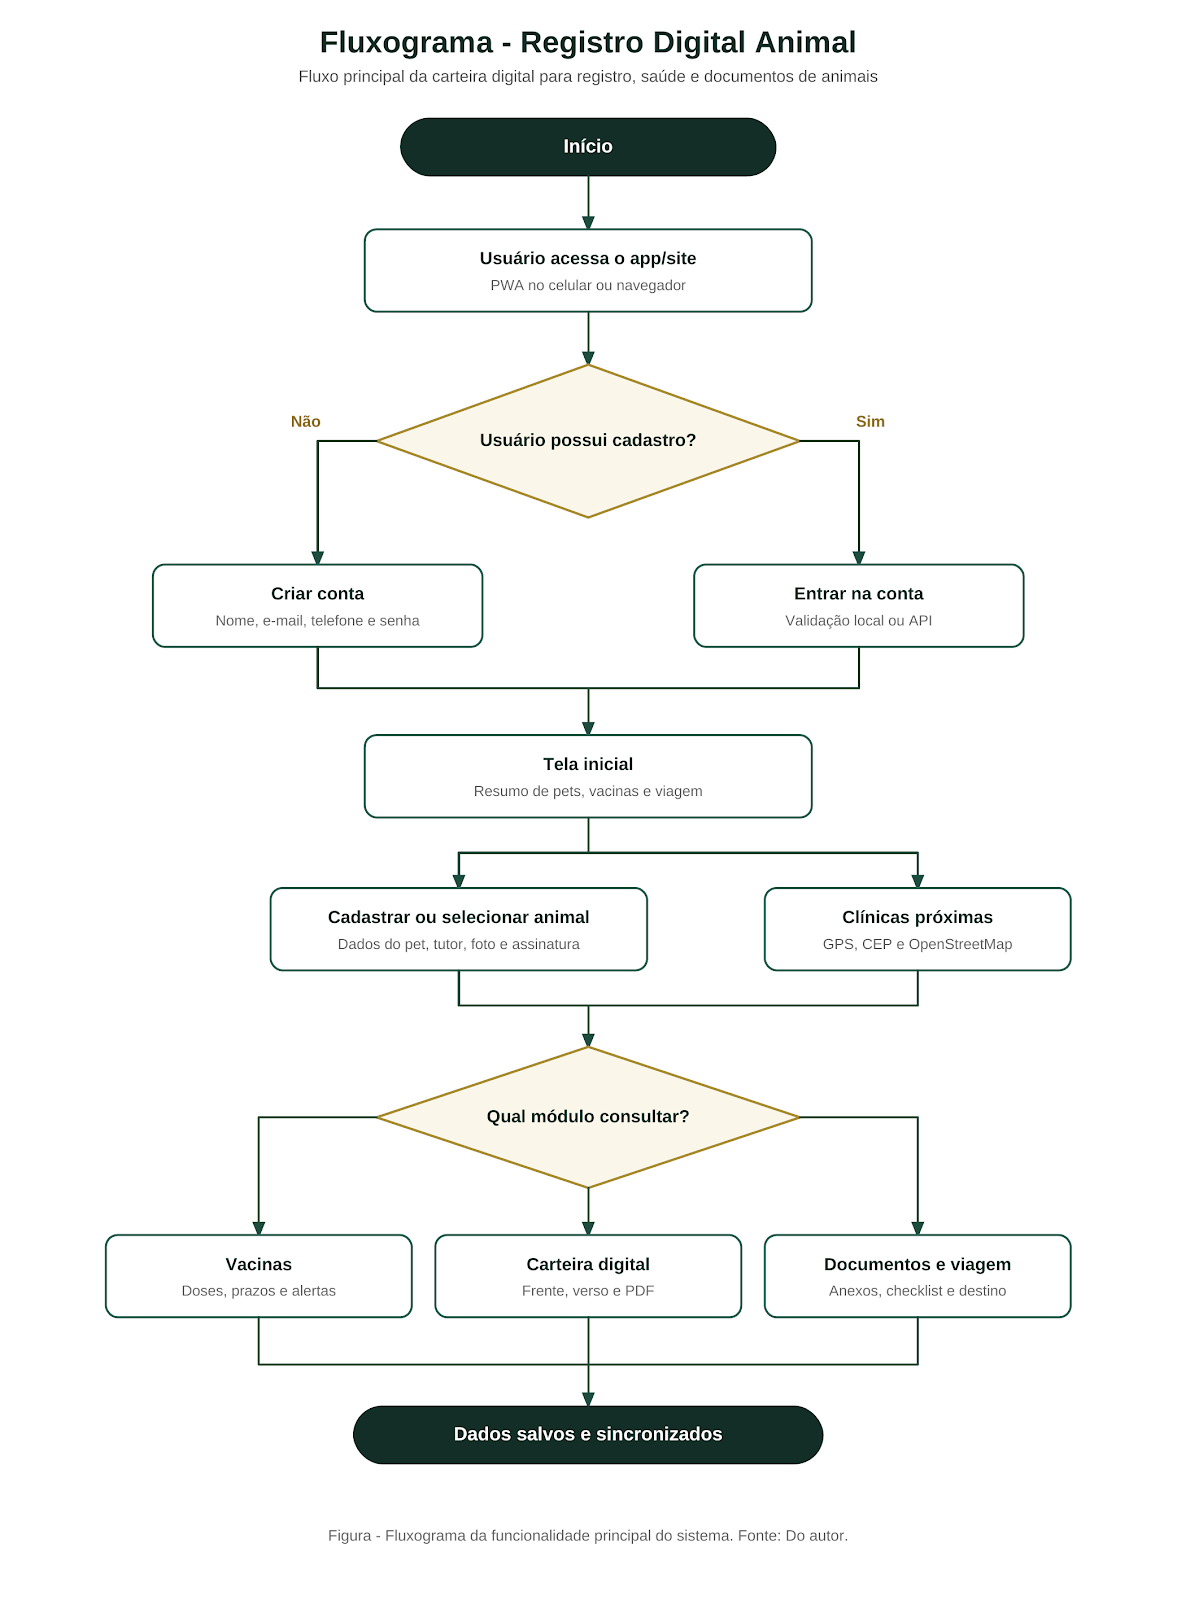
\includegraphics[scale=0.2]{Figs/fluxograma-registro-digital-animal.png}

\vspace{-0.2cm}
\begin{minipage}{\textwidth}
\footnotesize\raggedright Fonte: Elaborado pelo autor com auxílio do Codex GPT-5.5 (2026).
\end{minipage}
\end{figure}

No fluxo apresentado, o tutor acessa a aplicação por um navegador ou pela PWA instalada no dispositivo. As ações realizadas na interface são encaminhadas à API REST, responsável por processar as requisições, aplicar as regras do sistema e realizar as operações necessárias no banco de dados. As integrações externas são acionadas conforme a funcionalidade utilizada, enquanto os mecanismos de armazenamento local e sincronização permitem manter informações essenciais disponíveis em situações de conectividade limitada ou ausente.

Além do fluxo funcional, a Figura~\ref{fig:arquitetura_tecnologias_sistema} apresenta uma visão consolidada das tecnologias empregadas no desenvolvimento, na implantação e nos testes do sistema. O diagrama organiza os recursos utilizados nas camadas de \textit{frontend}, PWA e funcionamento offline, \textit{backend}, banco de dados, infraestrutura de hospedagem, integrações externas e ambiente de testes.

\begin{figure}[htbp]
\captionsetup{justification=raggedright,singlelinecheck=false,format=hang}
\caption{Arquitetura e tecnologias utilizadas no sistema Registro Digital Animal}
\label{fig:arquitetura_tecnologias_sistema}
\centering
\vspace{-0.2cm}
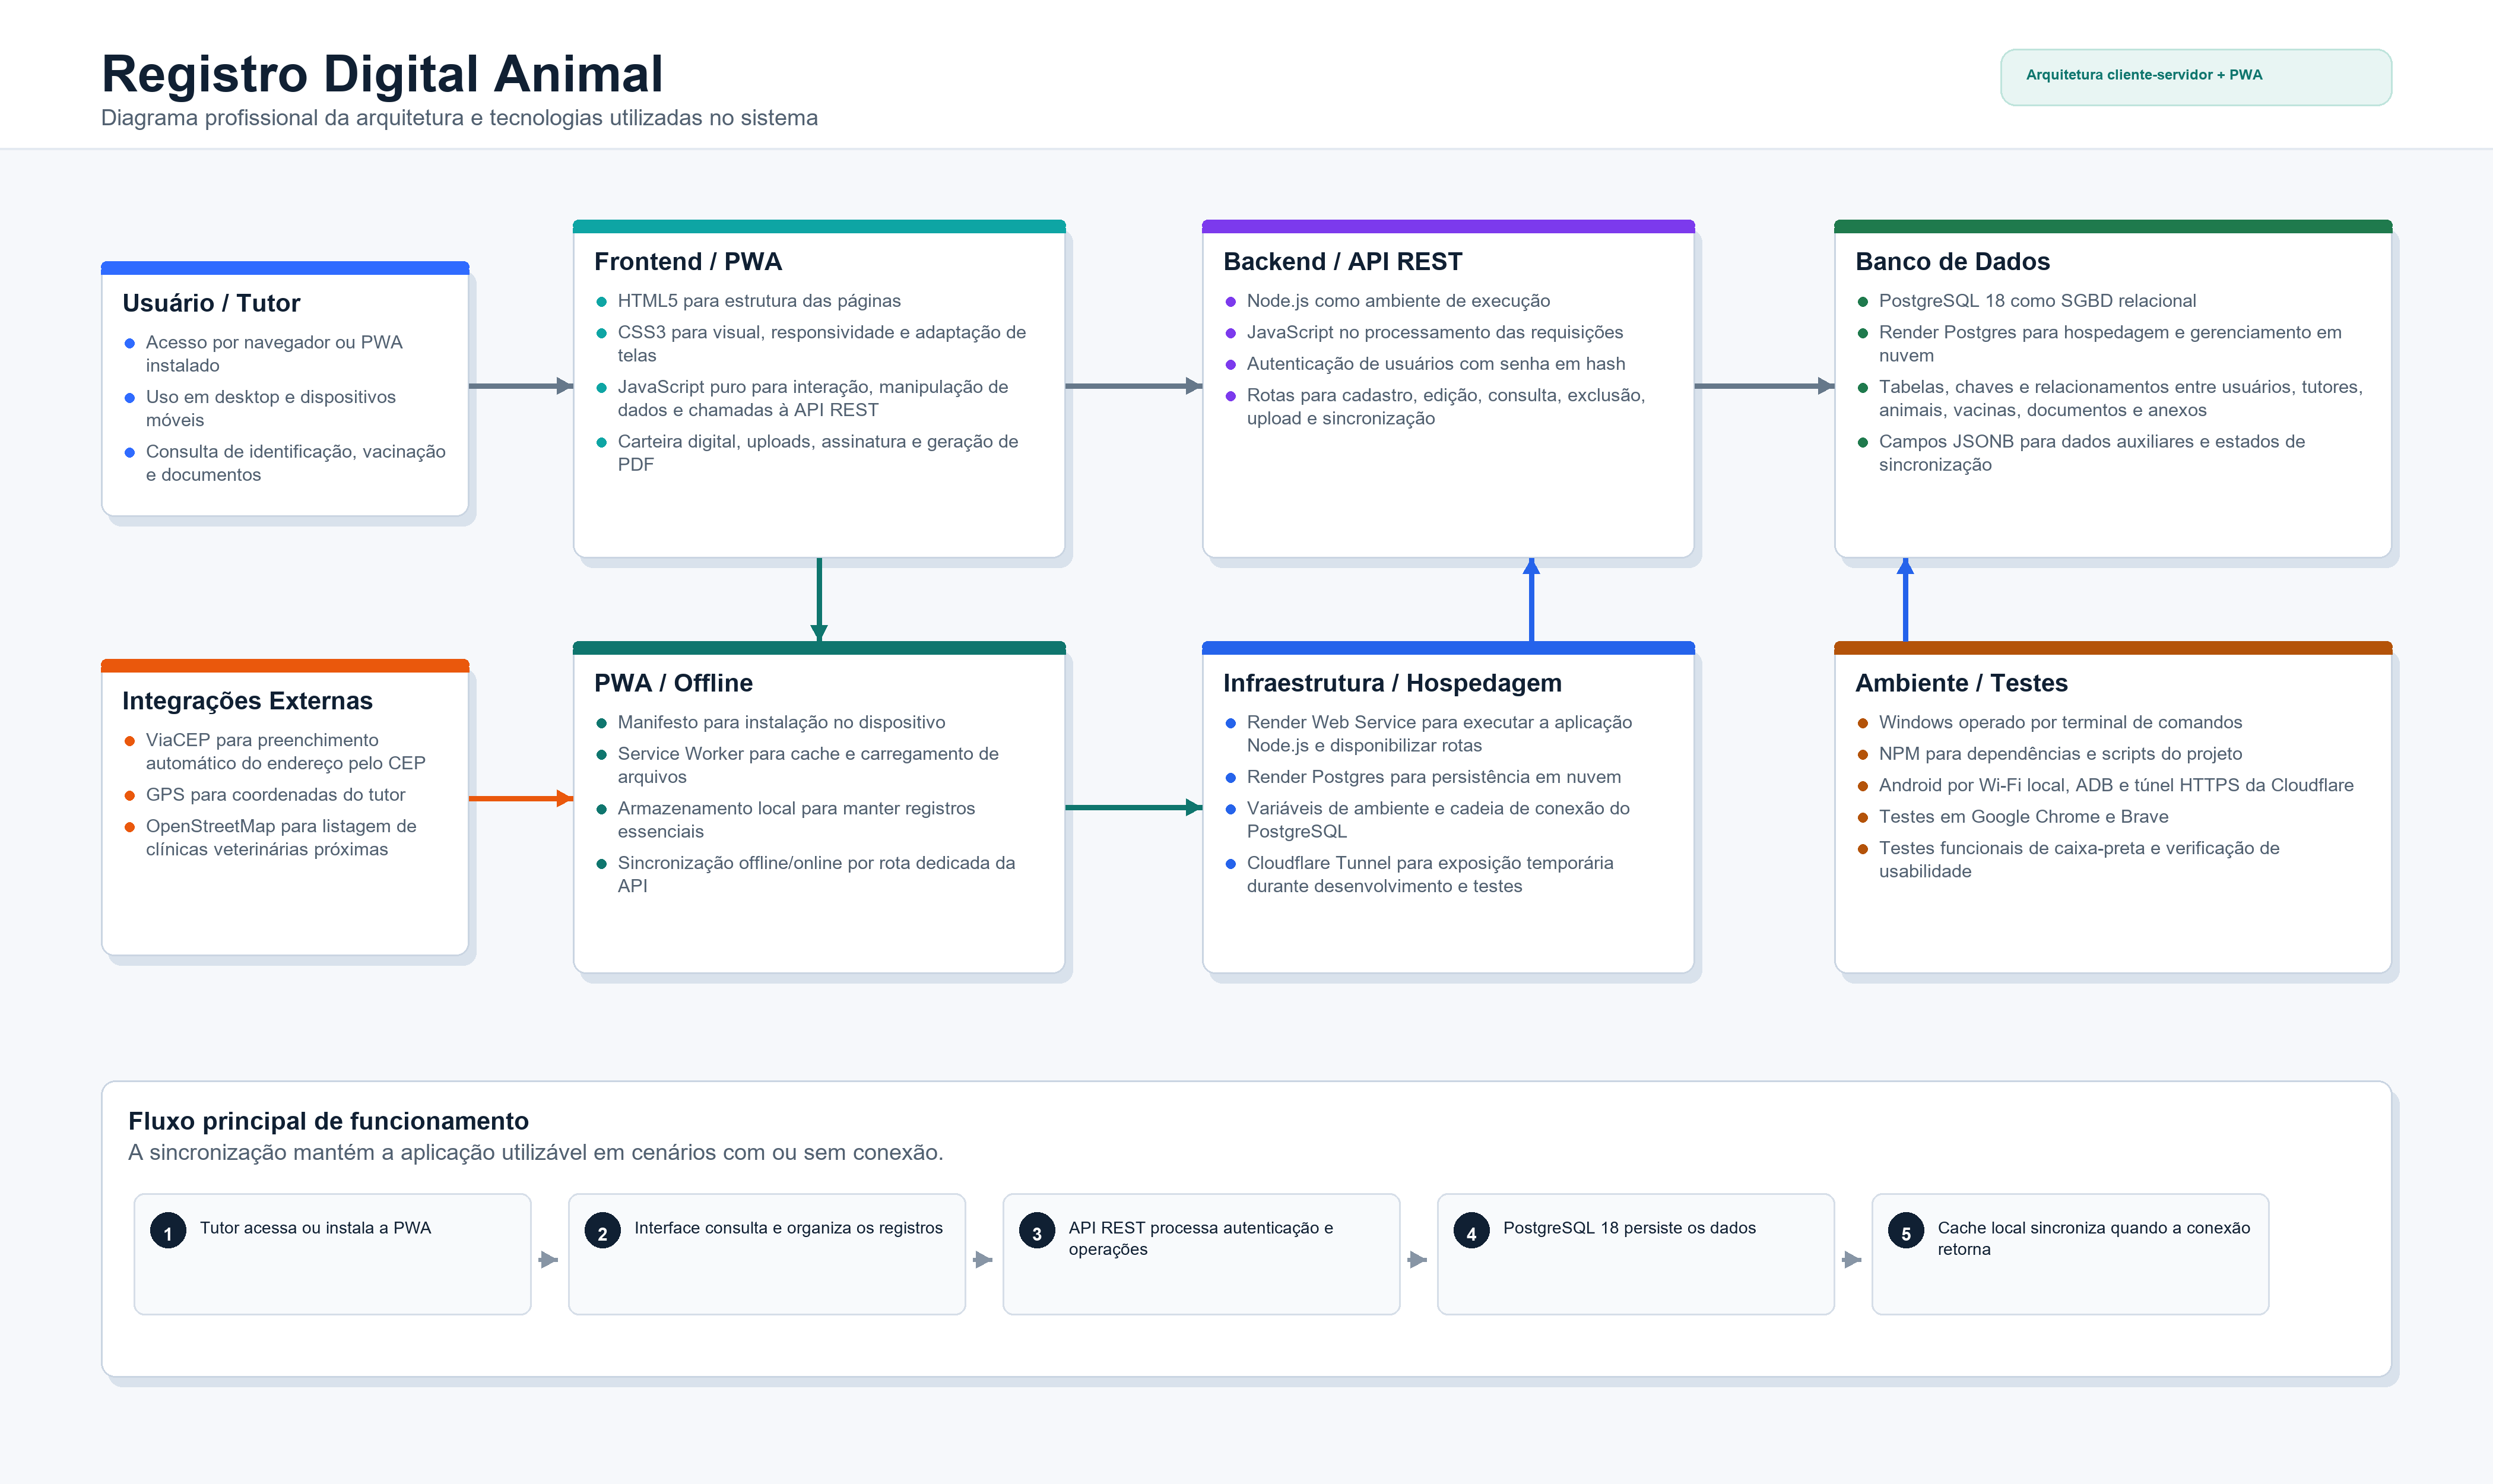
\includegraphics[width=\textwidth]{Figs/Registro_Digital_Animal_Diagrama.png}

\vspace{-0.2cm}
\begin{minipage}{\textwidth}
\footnotesize\raggedright Fonte: Elaborado pelo autor.
\end{minipage}
\end{figure}

No \textit{frontend}, foram utilizados HTML5, CSS3 e JavaScript puro, enquanto os recursos de PWA foram implementados por meio de manifesto, \textit{service worker}, \textit{cache} e armazenamento local. O \textit{backend} foi desenvolvido em JavaScript sobre o ambiente Node.js e organizado como uma API REST, com o NPM utilizado no gerenciamento das dependências e na execução dos scripts do projeto. A persistência das informações foi realizada no PostgreSQL 18, hospedado no Render Postgres, e a aplicação foi disponibilizada por meio de um Render Web Service.

As integrações externas incluíram a API ViaCEP, utilizada no preenchimento automático de endereços, e os recursos de GPS e OpenStreetMap, empregados na localização de clínicas veterinárias próximas ao tutor. Durante o desenvolvimento e os testes, foram utilizados o sistema operacional Windows, os navegadores Google Chrome e Brave, dispositivos Android, rede local Wi-Fi, Android Debug Bridge (ADB) e túnel HTTPS da Cloudflare.

A aplicação foi composta por módulos voltados ao gerenciamento das informações do tutor e do animal. O módulo de usuários permitiu o cadastro e a autenticação na plataforma via API com senhas armazenadas em formato de \textit{hash}. O módulo de animais possibilitou registrar e editar os dados de identificação do pet, incluindo o \textit{upload} de foto e o preenchimento automático do endereço a partir da consulta do CEP por meio da API ViaCEP, permanecendo sob responsabilidade do usuário o preenchimento do número e do complemento.

Além disso, o sistema contou com uma carteira digital do animal visualizável em formato frente e verso, recursos para captura de assinatura digital diretamente na aplicação, \textit{upload} de documentos do pet em formato de imagem ou PDF e geração ou \textit{download} da carteira e de seus anexos compilados em formato PDF. Para auxiliar em situações de emergência e localização, a aplicação integrou a geolocalização por GPS do tutor e os dados do OpenStreetMap para listar clínicas veterinárias próximas.

















\subsubsection{Banco de Dados}

O banco de dados foi organizado conforme as seis tabelas apresentadas na Figura~\ref{fig:diagrama_banco_dados}. A descrição de cada estrutura e de sua finalidade na aplicação é apresentada a seguir.

\begin{itemize}
    \item \textbf{\texttt{pet\_app\_users}}: armazena as informações de cadastro e autenticação dos usuários, incluindo identificador, nome, e-mail, e-mail normalizado, telefone, \textit{hash} da senha e datas de criação e atualização. Seu identificador associa os registros ao usuário responsável.
    \item \textbf{\texttt{pet\_owners}}: mantém os dados do tutor vinculados ao usuário por \texttt{user\_id}, incluindo nome, CPF, telefone, e-mail, endereço, número, complemento, bairro, município, estado, CEP, coordenadas de localização e contato de emergência.
    \item \textbf{\texttt{pet\_pets}}: reúne os dados de identificação dos animais, associados ao usuário e identificados por \texttt{id}. Contempla nome, espécie, raça, sexo, nascimento, peso, cor, microchip, registro, temperamento, alergias, observações e cor de apresentação do perfil, além das datas de criação e atualização.
    \item \textbf{\texttt{pet\_vaccines}}: registra as vacinas relacionadas ao usuário e ao animal, por meio de \texttt{user\_id} e \texttt{pet\_id}. Contém identificador do registro, nome da vacina, dose, data de aplicação, data prevista para a próxima dose, clínica, veterinário, lote, observações e datas de criação e atualização.
    \item \textbf{\texttt{pet\_documents}}: organiza os documentos vinculados ao usuário e ao animal, armazenando título, categoria, data do documento, validade e observações. Também mantém os dados do anexo, como nome, tipo, tamanho, identificador de armazenamento, endereço do arquivo, indicadores e conteúdo do anexo, além das datas de envio, armazenamento, criação e atualização.
    \item \textbf{\texttt{pet\_travel\_plans}}: armazena o planejamento de viagem associado ao usuário e ao animal. Contempla destino, data da viagem, meio de transporte, identificação do animal selecionado, observações e data de atualização.
\end{itemize}











A Figura~\ref{fig:diagrama_banco_dados} apresenta o diagrama do banco de dados utilizado pela aplicação, incluindo as tabelas, os campos armazenados, os tipos de dados, as chaves e os relacionamentos existentes entre as estruturas.

\begin{figure}[htbp]
\captionsetup{
    justification=raggedright,
    singlelinecheck=false,
    format=hang
}
\caption{Diagrama relacional do banco de dados PostgreSQL da aplicação Registro Digital Animal}
\label{fig:diagrama_banco_dados}

\centering
\vspace{-0.2cm}

% Remove aproximadamente 38\% do espaço à direita
\adjustbox{
    Clip=0pt 0pt {.38\width} 0pt,
    width=.62\textwidth
}{
    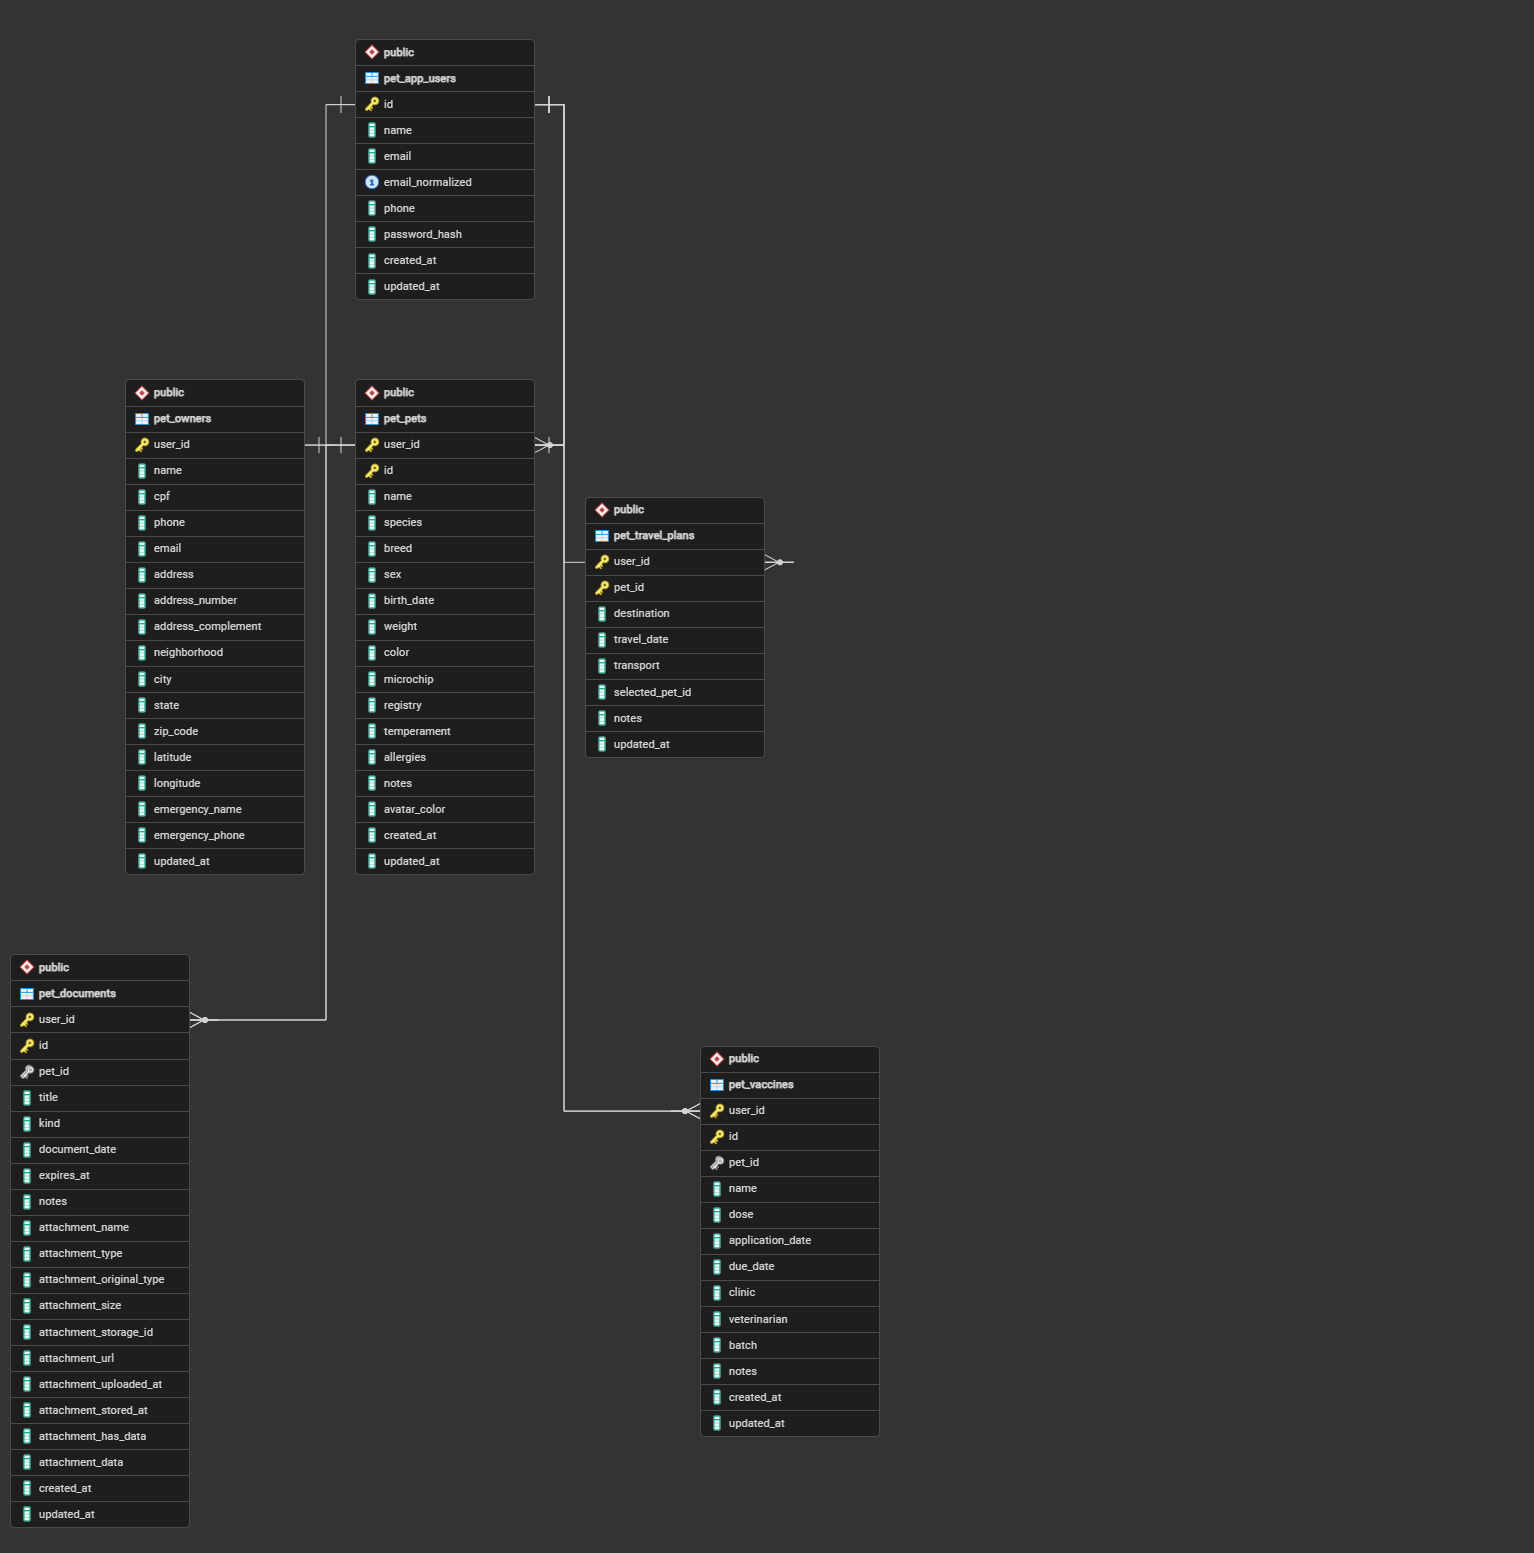
\includegraphics{Figs/Untitled.png}
}

\vspace{-0.2cm}
\begin{minipage}{\textwidth}
\footnotesize\raggedright
Fonte: Elaborado pelo autor.
\end{minipage}
\end{figure}







% \subsection{Metodologia de Avaliação}

% A avaliação da aplicação foi estruturada em duas etapas complementares. A primeira consistiu na realização de testes funcionais e de usabilidade do sistema, enquanto a segunda compreendeu uma pesquisa de campo com estabelecimentos e profissionais da área veterinária do estado de Santa Catarina. A pesquisa de campo encontra-se em andamento e tem como objetivo obter avaliações externas sobre a aplicação Registro Digital Animal, verificando a percepção de profissionais que atuam diretamente com cuidados relacionados à saúde animal e identificando possíveis melhorias, informações ausentes e funcionalidades consideradas relevantes para a utilização do sistema.

% Inicialmente, foram realizados testes funcionais de caixa-preta, nos quais se verificaram os comportamentos esperados do sistema sem análise direta de sua estrutura interna de código. Esses testes tiveram como finalidade confirmar se as funcionalidades implementadas estavam operando de acordo com os requisitos definidos para a aplicação. Foram avaliados o cadastro e a autenticação de usuários com armazenamento seguro das senhas por meio de \textit{hash}, o cadastro e a edição dos animais, a integração com o ViaCEP, a busca de estabelecimentos veterinários por meio de GPS e OpenStreetMap, a visualização e geração da carteira digital em PDF, o \textit{upload} de documentos e fotografias, a captura de assinatura digital, a sincronização de dados entre os modos offline e online por meio da API e a adaptação da interface PWA aos ambientes \textit{desktop} e móvel.

% Para cada funcionalidade, foram considerados cenários de utilização normal e situações de erro, verificando-se o comportamento apresentado pela aplicação, as mensagens fornecidas ao usuário e a correta manutenção dos dados. A avaliação também contemplou aspectos de usabilidade a partir da navegação pelos principais fluxos do sistema, considerando a clareza das telas, a facilidade de localização das informações, a organização dos elementos da carteira digital, a compreensão dos formulários e a prevenção de erros durante o preenchimento dos dados.

% Além dos testes realizados diretamente no sistema, foi iniciada uma pesquisa de campo com clínicas veterinárias e outros estabelecimentos relacionados à área veterinária. Essa etapa busca aproximar a avaliação da aplicação de um contexto real de utilização, permitindo coletar a opinião de profissionais que possuem contato cotidiano com tutores, animais, registros de vacinação, documentos clínicos e demais informações contempladas pelo aplicativo.

% A identificação dos estabelecimentos participantes foi realizada por meio de duas estratégias de busca. Para o município de Criciúma, Santa Catarina, foram localizadas clínicas veterinárias utilizando o Google Maps. A plataforma foi utilizada como ferramenta de apoio para identificar estabelecimentos da região e obter informações públicas de contato disponibilizadas pelos próprios negócios. A partir dessa busca, foram selecionadas clínicas veterinárias localizadas no município para posterior contato e apresentação da proposta de avaliação da aplicação.

% Com o objetivo de ampliar a abrangência geográfica da pesquisa para além de Criciúma, também foram realizadas buscas por estabelecimentos localizados em outras regiões do estado de Santa Catarina. Para essa etapa, foi utilizada a ferramenta de pesquisa avançada disponibilizada pelo site Casa dos Dados. A plataforma permitiu realizar consultas direcionadas a empresas cadastradas no estado, utilizando filtros relacionados à localização e à atividade desenvolvida pelos estabelecimentos. Dessa forma, foi possível identificar potenciais participantes distribuídos em diferentes municípios catarinenses e ampliar o alcance da avaliação para além do contexto local.

% A utilização dessas duas estratégias possibilitou constituir uma relação de possíveis participantes provenientes tanto do município de Criciúma quanto de outras localidades de Santa Catarina. A seleção não teve como finalidade produzir uma amostra probabilística representativa de todos os estabelecimentos veterinários do estado, mas obter avaliações de profissionais e empresas diretamente relacionados ao domínio de aplicação do sistema, capazes de fornecer contribuições técnicas e práticas para o aprimoramento da solução desenvolvida.

% Após a identificação dos estabelecimentos e a obtenção das informações públicas de contato, a abordagem foi realizada remotamente por meio do aplicativo WhatsApp. O contato inicial apresentou o pesquisador, informou que a aplicação estava sendo desenvolvida como parte de um Trabalho de Conclusão de Curso do curso de Ciência da Computação e explicou, de forma resumida, o objetivo do sistema e da avaliação proposta.

% Durante o convite, foi informado aos participantes que a aplicação tem como finalidade centralizar e facilitar o acesso a informações de identificação e saúde dos animais de estimação. Foram apresentadas as principais funcionalidades do sistema, incluindo o cadastro dos animais, o armazenamento das informações de vacinação, a organização de documentos relacionados ao pet, a carteira digital, os recursos voltados ao acesso às informações em diferentes dispositivos e outras funcionalidades relacionadas ao acompanhamento dos registros do animal.

% Aos estabelecimentos que demonstraram disponibilidade para participar da avaliação, foram encaminhadas orientações para acesso ao sistema e material explicativo destinado a demonstrar o funcionamento da aplicação. Esse procedimento foi adotado com o objetivo de permitir que os participantes conhecessem as funcionalidades disponíveis antes de apresentar suas opiniões, possibilitando uma avaliação baseada na interação ou na observação efetiva do sistema, e não somente em sua descrição textual.

% Após a apresentação e experimentação da aplicação, os participantes foram convidados a fornecer seu \textit{feedback} por meio do próprio contato realizado pelo WhatsApp. A avaliação buscou identificar principalmente a percepção dos profissionais em relação à utilidade das funcionalidades existentes, à organização das informações apresentadas, à adequação dos registros disponibilizados aos tutores e à possível existência de dados ou recursos considerados importantes para a rotina relacionada aos cuidados veterinários e que ainda não estivessem contemplados pelo aplicativo.

% Também foram consideradas sugestões de novas funcionalidades, alterações nos campos existentes, modificações na apresentação das informações e observações relacionadas à utilização prática da aplicação. Dessa forma, a participação dos profissionais não foi limitada à confirmação do funcionamento técnico do sistema, mas buscou obter uma avaliação qualitativa baseada na experiência dos participantes com atividades relacionadas à saúde e ao atendimento de animais de estimação.

% O contato por WhatsApp também possibilitou a continuidade da comunicação com os estabelecimentos durante o período de avaliação. Nos casos em que o convite inicial não obteve resposta, puderam ser realizados contatos posteriores para verificar a disponibilidade do estabelecimento em participar da pesquisa, mantendo-se a participação de caráter voluntário. As respostas recebidas estão sendo registradas e organizadas para posterior análise.

% No momento de realização deste trabalho, a pesquisa de campo ainda se encontra em andamento. Novos estabelecimentos continuam sendo identificados e contatados tanto em Criciúma quanto em outros municípios de Santa Catarina. Consequentemente, a quantidade de participantes e o conjunto final de respostas poderão ser ampliados durante o período destinado à coleta de dados.

% Após o encerramento da etapa de coleta, os \textit{feedbacks} obtidos serão organizados de acordo com os principais aspectos avaliados, permitindo identificar recorrências, sugestões de melhoria, funcionalidades consideradas relevantes e possíveis limitações observadas pelos participantes. As informações resultantes dessa etapa serão apresentadas posteriormente na seção de Resultados e Discussão, juntamente com a análise dos testes funcionais e de usabilidade realizados na aplicação.

% \subsubsection{Procedimento dos Testes}

% Os testes foram executados em etapas. Inicialmente, verificaram-se o cadastro de usuários, o hash de senhas e a autenticação na API. Em seguida, testaram-se o cadastro dos pets, a busca automática de endereço por CEP e a inclusão de foto e assinatura digital. Na sequência, avaliaram-se o visualizador da carteira digital em frente e verso, o envio de documentos (imagens/PDF) e o exportador da carteira compilada em PDF.

% Analisou-se também o comportamento da aplicação em dispositivos móveis Android sob três modalidades de acesso: via rede local Wi-Fi, por conexão ADB via cabo USB e por acesso externo através do túnel HTTPS da Cloudflare. Em todas as abordagens de conexão, verificou-se que o sistema apresentou comportamento equivalente e consistente, garantindo o funcionamento das rotas, a responsividade da interface e a captura de coordenadas GPS para a busca de veterinárias próximas via OpenStreetMap. Por fim, testou-se a funcionalidade de persistência e sincronização dos dados offline com o banco PostgreSQL 18 hospedado no Render Postgres, verificando se as alterações realizadas localmente eram enviadas e armazenadas corretamente quando o servidor e a conexão com a internet retornavam à disponibilidade.

% Os resultados dos testes foram organizados de acordo com o comportamento observado em cada cenário, classificando as funcionalidades como aprovadas. Os testes confirmaram a plena conformidade das respostas do sistema e a validação satisfatória de todas as funcionalidades avaliadas.

\subsection{Metodologia de Avaliação}

A avaliação foi organizada em testes funcionais de caixa-preta, com observação de aspectos de usabilidade, e pesquisa de campo com profissionais veterinários. Os testes verificaram as respostas da aplicação às ações do usuário, enquanto a pesquisa reuniu percepções sobre a utilidade da solução.

\subsubsection{Procedimento e cenários dos testes}

Os testes foram executados em computadores com Windows, nos navegadores Google Chrome e Brave, e em dispositivos Android. O acesso móvel foi realizado por rede local Wi-Fi, depuração USB com Android Debug Bridge (ADB) e túnel HTTPS da Cloudflare. Para cada cenário, comparou-se o comportamento observado ao resultado esperado. A classificação Passou correspondeu à execução da tarefa prevista e à manutenção dos dados envolvidos. A observação de usabilidade considerou clareza das telas, navegação, organização das informações e preenchimento dos formulários.

Os 15 cenários foram identificados de F01 a F15, mantendo a correspondência com os resultados apresentados na Tabela~\ref{tab:testes_funcionais}:

\begin{itemize}
    \item \textbf{F01 -- Cadastro de usuário e armazenamento de senha com \textit{hash}}: Realizar o cadastro e verificar os dados persistidos e o armazenamento da senha em formato de hash.
    \item \textbf{F02 -- Autenticação do usuário e controle de sessão na API REST}: Efetuar o acesso e verificar a sessão e a restrição de acesso às rotas protegidas.
    \item \textbf{F03 -- Cadastro e edição de perfil de animal com \textit{upload} de foto}: Cadastrar e editar o animal, enviar uma fotografia e conferir os dados recuperados na interface.
    \item \textbf{F04 -- Preenchimento automático de endereço via API ViaCEP a partir do CEP}: Informar um CEP válido e conferir o preenchimento automático do endereço pela API ViaCEP.
    \item \textbf{F05 -- Captura e salvamento de assinatura digital no formulário}: Capturar e salvar a assinatura e verificar sua legibilidade e associação ao cadastro.
    \item \textbf{F06 -- Visualização interativa da carteira digital, com frente e verso}: Consultar a carteira e alternar entre frente e verso, conferindo os dados do tutor e do animal.
    \item \textbf{F07 -- \textit{Upload} e vinculação de documentos clínicos em imagem ou PDF}: Enviar documentos em imagem ou PDF e verificar a vinculação ao animal e a disponibilidade para consulta.
    \item \textbf{F08 -- Geração e exportação da carteira digital consolidada em PDF}: Gerar o PDF e conferir os dados cadastrais, vacinas, anexos e assinatura.
    \item \textbf{F09 -- Captura de coordenadas de geolocalização via GPS móvel}: Utilizar o GPS em Android e verificar a obtenção das coordenadas.
    \item \textbf{F10 -- Consulta de clínicas veterinárias próximas via OpenStreetMap}: Consultar os estabelecimentos no OpenStreetMap a partir da localização obtida.
    \item \textbf{F11 -- Responsividade e navegação em \textit{desktop} nos navegadores Chrome e Brave}: Navegar pelos principais fluxos em Chrome e Brave e verificar a adaptação às dimensões de tela.
    \item \textbf{F12 -- Acesso móvel em Android via Wi-Fi, ADB e túnel Cloudflare}: Comparar o acesso em Android por Wi-Fi, ADB e túnel HTTPS da Cloudflare.
    \item \textbf{F13 -- Armazenamento e execução de \textit{cache} pelo \textit{Service Worker}}: Verificar o armazenamento e o carregamento dos recursos da PWA pelo Service Worker.
    \item \textbf{F14 -- Acesso e consulta offline aos dados da carteira e das vacinas}: Interromper a conectividade e consultar os dados da carteira e das vacinas previamente armazenados.
    \item \textbf{F15 -- Sincronização offline-online de registros no banco PostgreSQL}: Realizar alterações locais sem conexão, restabelecer a conectividade e conferir o envio à API e a persistência no PostgreSQL.
\end{itemize}

Para registrar os problemas de usabilidade observados, adotou-se a escala de severidade de Nielsen: 0 (não é problema), 1 (problema cosmético), 2 (problema menor), 3 (problema maior) e 4 (problema catastrófico). Os resultados funcionais e as classificações de severidade são apresentados na seção de Resultados e Discussão.

\subsubsection{Procedimento da pesquisa de campo}

A pesquisa de campo envolveu clínicas veterinárias e estabelecimentos do setor em Santa Catarina, identificados pelo Google Maps em Criciúma e pela plataforma Casa dos Dados nos demais municípios. A seleção buscou profissionais relacionados ao domínio de aplicação, sem constituir uma amostra probabilística representativa do estado. O contato foi realizado remotamente via WhatsApp, com apresentação do pesquisador, do objetivo do trabalho e das funcionalidades da aplicação. Aos interessados foram encaminhados orientações de acesso e material explicativo para apoiar a experimentação ou observação do sistema.

As percepções foram coletadas pelo mesmo canal de contato e organizadas por aspectos de utilidade, acesso às informações, funcionamento offline, documentação digital e sugestões de melhoria. A análise qualitativa buscou identificar recorrências e necessidades de aprimoramento. Os retornos obtidos são apresentados na seção de Resultados e Discussão.

\begingroup
\makeatletter
% Alinha a continuação da legenda ao título, após o número da tabela.
\@ifundefined{captionsetup}{%
  \long\def\@makecaption#1#2{%
    \vskip\abovecaptionskip
    {\normalsize\normalfont
      \sbox\@tempboxa{#1\space-\space}%
      \raggedright
      \hyphenpenalty=10000
      \hangindent=\wd\@tempboxa
      \hangafter=1
      \noindent#1\space-\space#2\par}%
    \vskip\belowcaptionskip}%
}{%

  \captionsetup[table]{format=hang,justification=raggedright,
    singlelinecheck=false,labelsep=space,font=normalsize,
    labelfont=normalfont,textfont=normalfont,skip=6pt}%
}
\makeatother

\section{RESULTADOS E DISCUSSÃO}

Nesta seção são apresentados e discutidos os resultados obtidos na avaliação da aplicação \textbf{Registro Digital Animal}. A validação foi organizada em duas frentes complementares: a execução de testes funcionais de caixa-preta, com observação de aspectos de usabilidade, e a análise qualitativa das percepções coletadas junto a estabelecimentos e profissionais da área veterinária do estado de Santa Catarina. Dessa forma, buscou-se verificar não apenas o funcionamento técnico da solução, mas também sua aderência a necessidades reais do contexto de acompanhamento e identificação de animais.

\subsection{Testes funcionais e avaliação de usabilidade}

A Tabela~\ref{tab:testes_funcionais} apresenta os resultados dos 15 cenários definidos na seção de Materiais e Métodos, mantendo seus identificadores e as respectivas classificações de severidade.



\begin{table}[htbp]
\centering
\caption{Resultados dos testes funcionais e de usabilidade do sistema}
\label{tab:testes_funcionais}
\par\vspace{4pt}
\small
\setlength{\tabcolsep}{4pt}
\renewcommand{\arraystretch}{1.15}
\begin{tabular}{@{}p{0.07\linewidth} p{\dimexpr0.64\linewidth-6\tabcolsep\relax} p{0.13\linewidth} p{0.16\linewidth}@{}}
\hline
\textbf{ID} & \textbf{Cenário de teste avaliado} & \textbf{Resultado} & \textbf{Severidade} \\
\hline
F01 & Cadastro de usuário e armazenamento de senha com \textit{hash} & Passou & 0 \\
F02 & Autenticação do usuário e controle de sessão na API REST & Passou & 0 \\
F03 & Cadastro e edição de perfil de animal com \textit{upload} de foto & Passou & 0 \\
F04 & Preenchimento automático de endereço via API ViaCEP a partir do CEP & Passou & 0 \\
F05 & Captura e salvamento de assinatura digital no formulário & Passou & 0 \\
F06 & Visualização interativa da carteira digital, com frente e verso & Passou & 0 \\
F07 & \textit{Upload} e vinculação de documentos clínicos em imagem ou PDF & Passou & 0 \\
F08 & Geração e exportação da carteira digital consolidada em PDF & Passou & 0 \\
F09 & Captura de coordenadas de geolocalização via GPS móvel & Passou & 0 \\
F10 & Consulta de clínicas veterinárias próximas via OpenStreetMap & Passou & 0 \\
F11 & Responsividade e navegação em \textit{desktop} nos navegadores Chrome e Brave & Passou & 0 \\
F12 & Acesso móvel em Android via Wi-Fi, ADB e túnel Cloudflare & Passou & 0 \\
F13 & Armazenamento e execução de \textit{cache} pelo \textit{Service Worker} & Passou & 0 \\
F14 & Acesso e consulta offline aos dados da carteira e das vacinas & Passou & 0 \\
F15 & Sincronização offline-online de registros no banco PostgreSQL & Passou & 0 \\
\hline
\end{tabular}
\par\vspace{2pt}
\begin{minipage}{\linewidth}
\footnotesize\raggedright
Fonte: Elaborado pelo autor.
\end{minipage}
\end{table}

Conforme apresentado na Tabela~\ref{tab:testes_funcionais}, todos os cenários avaliados foram concluídos com êxito, resultando em taxa de sucesso de 100\% nos testes executados. Nenhum dos cenários recebeu classificação de severidade superior a 0, o que indica que, no ambiente de validação utilizado, não foram observadas falhas funcionais ou problemas de usabilidade capazes de comprometer a execução das tarefas previstas.

Nos cenários F01 e F02, referentes à autenticação e ao controle de acesso, verificou-se que a API REST realizou corretamente o cadastro de usuários, armazenando as senhas em formato de \textit{hash}, sem persistência de credenciais em texto puro. Também foi confirmada a restrição de acesso às rotas protegidas, o que contribui para a segurança dos dados pessoais e dos registros dos animais.

No módulo de gestão do animal, contemplado pelos cenários F03 a F05, o formulário de cadastro apresentou comportamento consistente durante a inserção e edição das informações. A integração com a API ViaCEP reduziu o preenchimento manual de dados de endereço, ao completar automaticamente logradouro, bairro, cidade e estado após a inserção de um CEP válido. A captura da assinatura digital também foi executada corretamente, mantendo a legibilidade do traço e sua associação ao cadastro do animal.

Em relação à carteira digital e aos documentos, avaliados nos cenários F06 a F08, a aplicação permitiu a visualização organizada das informações do animal e do tutor, incluindo a alternância entre frente e verso da carteira. O envio de documentos clínicos em imagem ou PDF funcionou adequadamente, e a exportação consolidada em PDF reuniu os principais dados cadastrais, registros de vacinação, anexos e assinatura digital em um único arquivo. Esse resultado reforça a proposta do sistema como alternativa digital à caderneta física, especialmente em situações nas quais o tutor precisa apresentar rapidamente o histórico do animal.

Os testes de mobilidade e geolocalização, correspondentes aos cenários F09 a F12, demonstraram que a aplicação manteve comportamento estável em diferentes formas de acesso. Em dispositivos Android, a captura de coordenadas por GPS e a integração com o OpenStreetMap possibilitaram a listagem de estabelecimentos veterinários próximos à localização do usuário. Além disso, a execução em rede Wi-Fi local, depuração via ADB e acesso por túnel HTTPS com Cloudflare apresentou funcionamento equivalente, sem inconsistências relevantes de navegação ou renderização da interface.

Por fim, os cenários F13 a F15 validaram os recursos de funcionamento offline e sincronização posterior. O \textit{Service Worker} e os mecanismos de \textit{cache} permitiram que a aplicação permanecesse acessível mesmo na ausência de conexão com a internet, garantindo a consulta às informações essenciais da carteira e dos registros de vacinação já salvos no dispositivo. Quando a conectividade foi restabelecida, os registros pendentes foram enviados à API REST e persistidos no banco PostgreSQL, evidenciando a viabilidade do uso da aplicação em contextos de mobilidade, atendimento externo ou instabilidade de rede.

Embora os resultados tenham sido positivos, ressalta-se que os testes foram realizados em um conjunto controlado de cenários e dispositivos. Assim, avaliações futuras com maior diversidade de usuários, navegadores, modelos de aparelhos e condições de conectividade podem ampliar a confiabilidade da validação e revelar necessidades adicionais de aprimoramento.

\subsection{Pesquisa de campo com profissionais veterinários}

Os retornos da pesquisa de campo foram organizados nos aspectos apresentados na Tabela~\ref{tab:resumo_qualitativo}, conforme o procedimento descrito em Materiais e Métodos.

A Tabela~\ref{tab:resumo_qualitativo} sintetiza os principais aspectos mencionados pelos participantes durante a avaliação.

\begin{table}[htbp]
\centering
\caption{Síntese da avaliação qualitativa recebida dos estabelecimentos veterinários}
\label{tab:resumo_qualitativo}
\par\vspace{4pt}
\small
\setlength{\tabcolsep}{5pt}
\renewcommand{\arraystretch}{1.15}
\begin{tabular}{@{}p{\dimexpr0.31\linewidth-\tabcolsep\relax} p{\dimexpr0.69\linewidth-\tabcolsep\relax}@{}}
\hline
\textbf{Aspecto avaliado} & \textbf{Percepção e observações dos participantes} \\
\hline
Organização do histórico & Avaliada de forma positiva, pois contribui para reduzir a perda, o esquecimento ou a rasura de registros vacinais físicos por parte dos tutores. \\
Praticidade e acessibilidade & Considerada adequada pela facilidade de consulta das informações no celular, tanto em atendimentos de rotina quanto em situações de urgência. \\
Funcionamento offline & Destacado como recurso relevante para deslocamentos, eventos externos, áreas com instabilidade de sinal e momentos em que a clínica não dispõe de conexão confiável. \\
Carteira em PDF e assinatura digital & Apontada como funcionalidade útil para apresentação do histórico de vacinas em viagens, hospedagens, atendimentos e demais situações que exijam comprovação documental. \\
Sugestões de aprimoramento & Recomendada a inclusão futura de alertas de retorno, lembretes automáticos de próximas doses e notificações relacionadas ao acompanhamento preventivo do animal. \\
\hline
\end{tabular}
\par\vspace{2pt}
\begin{minipage}{\linewidth}
\footnotesize\raggedright
Fonte: Elaborado pelo autor.
\end{minipage}
\end{table}

Os retornos obtidos indicam boa aceitação da proposta do \textbf{Registro Digital Animal}, especialmente pela possibilidade de centralizar em um único ambiente informações que, no modelo tradicional, costumam ficar dispersas em cadernetas físicas, comprovantes impressos, mensagens e documentos avulsos. O ponto mais enfatizado pelos participantes foi a organização do histórico vacinal, uma vez que a perda ou o esquecimento da caderneta física é uma ocorrência recorrente no atendimento veterinário.

A disponibilidade da aplicação em formato PWA também foi percebida como um diferencial, pois dispensa instalação por lojas de aplicativos e permite acesso direto pelo navegador ou por atalho na tela inicial do dispositivo. Esse aspecto favorece a adoção por tutores com diferentes níveis de familiaridade tecnológica, além de facilitar o acesso em situações de consulta, emergência, viagem ou hospedagem pet.

Outro ponto relevante foi a exportação da carteira em PDF, associada à assinatura digital e aos anexos clínicos. Essa funcionalidade aproxima o sistema de uma documentação mais completa e compartilhável, permitindo que o tutor apresente informações consolidadas quando solicitado. Na perspectiva dos profissionais consultados, esse recurso pode contribuir para reduzir falhas de comunicação entre tutor, clínica, hospedagem, transporte e demais serviços relacionados ao cuidado animal.

As sugestões de aprimoramento concentraram-se principalmente na inclusão de lembretes automáticos de vacinação e alertas de retorno. Essa recomendação evidencia que, além de registrar informações, o sistema pode evoluir para apoiar o acompanhamento preventivo do animal, auxiliando tutores e profissionais na manutenção de cuidados recorrentes. Portanto, os resultados da pesquisa de campo reforçam a relevância prática da solução e apontam caminhos para futuras versões da aplicação.

\endgroup

\section{Conclusão}
%Parte final do artigo, onde são apresentadas as conclusões correspondentes aos objetivos e as hipóteses. Deve ser breve, devendo apresentar recomendações e sugestões para trabalhos futuros.

\bibliographystyle{abntex2-unesc}
\renewcommand{\refname}{REFERÊNCIAS}
\bibliography{referencias} % arquivo referencias.bib que contém as referências bibliográficas utilizadas no artigo

%\setcounter{section}{}{} \label{app_a} % reset to start Attachment A
\renewcommand{\thesection}{APÊNDICE \Alph{section}}
\section{}
%São documentos elaborados pelo autor que servem como fundamentação (mapas, leis, estatutos). Deve ser precedido da palavra Apendice, identificada por letras maiúsculas consecutivas, travessão e pelo respectivo título. Utilizam-se letras maiúsculas dobradas quando esgotadas as letras do alfabeto. 



%\setcounter{section}{}{} \label{anex_a} % reset to start Attachment A
\renewcommand{\thesection}{Anexo \Alph{section}}
\section{}
%São documentos não elaborados pelo autor que servem como fundamentação (mapas, leis, estatutos). Deve ser precedido da palavra ANEXO, identificada por letras maiúsculas consecutivas, travessão e pelo respectivo título. Utilizam-se letras maiúsculas dobradas quando esgotadas as letras do alfabeto. 




\end{document}